\documentclass[tikz]{standalone}
\usepackage{tikz}
\usepackage{standalone}
\begin{document}	
	
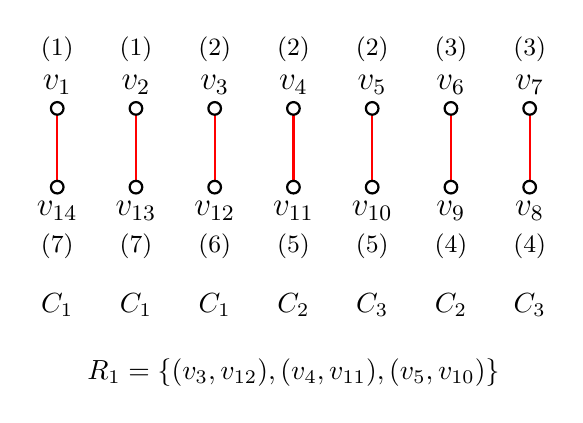
\begin{tikzpicture}
%\draw [help lines] (-1,-1) grid (9, 10);

\draw [thick, red] (1,2.5) -- (1,3.5);
\draw [thick, red] (2,2.5) -- (2,3.5);
\draw [thick, red] (3,2.5) -- (3,3.5);
\draw [thick, red] (4,2.5) -- (4,3.5);
\draw [thick, red] (5,2.5) -- (5,3.5);
\draw [thick, red] (6,2.5) -- (6,3.5);
\draw [thick, red] (7,2.5) -- (7,3.5);

\draw [fill=white, thick] (1,2.5) circle [radius = 0.08];
\draw [fill=white, thick] (2,2.5) circle [radius = 0.08];
\draw [fill=white, thick] (3,2.5) circle [radius = 0.08];
\draw [fill=white, thick] (4,2.5) circle [radius = 0.08];
\draw [fill=white, thick] (5,2.5) circle [radius = 0.08];
\draw [fill=white, thick] (6,2.5) circle [radius = 0.08];
\draw [fill=white, thick] (7,2.5) circle [radius = 0.08];
\draw [fill=white, thick] (1,3.5) circle [radius = 0.08];
\draw [fill=white, thick] (2,3.5) circle [radius = 0.08];
\draw [fill=white, thick] (3,3.5) circle [radius = 0.08];
\draw [fill=white, thick] (4,3.5) circle [radius = 0.08];
\draw [fill=white, thick] (5,3.5) circle [radius = 0.08];
\draw [fill=white, thick] (6,3.5) circle [radius = 0.08];
\draw [fill=white, thick] (7,3.5) circle [radius = 0.08];

\node at (1,2.2) {\large{$v_{14}$}};
\node at (2,2.2) {\large{$v_{13}$}};
\node at (3,2.2) {\large{$v_{12}$}};
\node at (4,2.2) {\large{$v_{11}$}};
\node at (5,2.2) {\large{$v_{10}$}};
\node at (6,2.2) {\large{$v_9$}};
\node at (7,2.2) {\large{$v_8$}};

\node at (1,1.75) {\small{(7)}};
\node at (2,1.75) {\small{(7)}};
\node at (3,1.75) {\small{(6)}};
\node at (4,1.75) {\small{(5)}};
\node at (5,1.75) {\small{(5)}};
\node at (6,1.75) {\small{(4)}};
\node at (7,1.75) {\small{(4)}};

\node at (1,3.8) {\large{$v_1$}};
\node at (2,3.8) {\large{$v_2$}};
\node at (3,3.8) {\large{$v_3$}};
\node at (4,3.8) {\large{$v_4$}};
\node at (5,3.8) {\large{$v_5$}};
\node at (6,3.8) {\large{$v_6$}};
\node at (7,3.8) {\large{$v_7$}};

\node at (1,4.25) {\small{(1)}};
\node at (2,4.25) {\small{(1)}};
\node at (3,4.25) {\small{(2)}};
\node at (4,4.25) {\small{(2)}};
\node at (5,4.25) {\small{(2)}};
\node at (6,4.25) {\small{(3)}};
\node at (7,4.25) {\small{(3)}};




\node at (1,1) {$C_1$};
\node at (2,1) {$C_1$};
\node at (3,1) {$C_1$};
\node at (4,1) {$C_2$};
\node at (5,1) {$C_3$};
\node at (6,1) {$C_2$};
\node at (7,1) {$C_3$};

\node at (4,0.15) {$R_1 = \{(v_3, v_{12}), (v_4, v_{11}), (v_5, v_{10})\}$};






\end{tikzpicture}
	
\end{document}
